% \documentclass[12pt]{article}

%%v helpful MIT exam schema, see http://www-math.mit.edu/~psh/exam/examdoc.pdf
 \documentclass[9pt]{exam} 
% \qformat{\textbf{Question \thequestion}\quad \thepoints\hfill } % Large depth to make space}
 \renewcommand{\thesubpart}{(\roman{subpart})}
 \renewcommand{\subpartlabel}{\thesubpart}
 \footer{}{}{Page \thepage\ de \numpages}
\addpoints
\pointsinmargin \marginpointname{ points}
% \boxedpoints
\renewcommand{\questionshook}{\setlength{\itemsep}{0.2cm}}
\renewcommand{\partshook}{
	\setlength{\itemsep}{0.1cm}
}


\usepackage{cmbright}

\pagestyle{empty} %for handouts
\addtolength{\jot}{2em} % this makes all formulae a bit more spaced vertically for handouts
\setlength{\parindent}{0pt} %we're not writing a novel
%\renewcommand{\arraystretch}{2} %makes tables taller, so easier to write in

\usepackage[fleqn]{amsmath}
\usepackage{amssymb} %standard classy maths symbols
\usepackage[a4paper, margin=1in]{geometry} %makes it easy to specify where to put stuff on the page

\usepackage{siunitx} %v handy way of getting SI units to typeset correctly...
% \sisetup{locale = FR} %... and now it will use a comma for decimals

\usepackage[utf8]{inputenc}

% \usepackage[french]{babel} % frenchify everything (e.g. a Table becomes a Tableau)
% \usepackage{lmodern} % font with nicer French characters than standard
% \usepackage{textcomp} % and more help for special characters

\usepackage{tcolorbox} % basic but good package for boxes around text
\tcbset{colback=black!5!white}
% \usepackage{color} % colours
%\newcommand{\fillin}{\color{black!1!white}} %makes the text disappear
%\definecolor{fillin}{rgb} {1.00,1.00,1.00}
%\renewcommand{\fillin}{\color{blue}} \definecolor{fillin}{rgb} {0.00,0.00,1.00} %makes the filling in text appear (in blue)

\usepackage{enumitem} % can change the labels on lists, items, enumerates
\usepackage{setspace}

\usepackage{tikz, pgfplots} % interval diagrams, sets, etc.
%\usetikzlibrary{calc,trees,positioning,arrows,fit,shapes}
\usetikzlibrary{arrows.meta}

\begin{document}

\textbf{Name:} \dotfill

\vspace{-2mm}

\begin{questions}


\question[7] Giving an example if necessary, is $f\ldots$

\begin{parts}

\begin{minipage}[t]{0.55\textwidth}
\vspace{1mm}

\part a function? \dotfill

\

\part  injective? \dotfill

\

\part surjective? \dotfill

\

\part bijective?\dotfill
\end{minipage}
\hspace{5mm}
\begin{minipage}[t]{0.4\textwidth}
\vspace{-8mm}


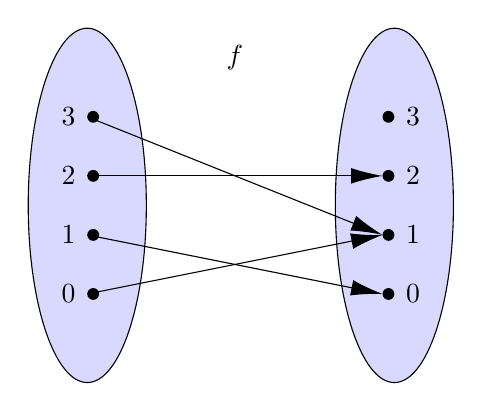
\begin{tikzpicture}[scale=0.75]

\draw[fill=blue!15] (1,1.5) ellipse (1cm and 3cm); 
\foreach \x in {0, 1, 2, 3}{
\fill (1.1, \x) circle (1mm) node[left=1mm] {$\x$};
}


\draw[fill=blue!15] (6.2,1.5) ellipse (1cm and 3cm); 
\foreach \x in {0, 1, 2, 3}{
\fill (6.1, \x) circle (1mm) node[right=1mm] {$\x$};
}

\draw[-{Latex[length=4mm,width=2mm]}] (1,0)--(6,1);
\draw[-{Latex[length=4mm,width=2mm]}] (1,1)--(6,0);
\draw[-{Latex[length=4mm,width=2mm]}] (1,2)--(6,2);
\draw[-{Latex[length=4mm,width=2mm]}] (1,3)--(6,1);

\node at (3.5, 4) {$f$};
\end{tikzpicture}


\end{minipage}

\part Work out $(f\circ f)(3)$
\fillwithdottedlines{8mm}

\fullwidth{We can also define $f$ as a set of ordered pairs $\big\{ (0, 1), (1, 0), (2, 2), (3, 1) \big\}$.}
\part Give a new set of ordered pairs for a restriction of $f$ which is a bijection.
\fillwithdottedlines{10mm}

\end{parts}

\question[7] Define $g : x \mapsto (x-2)^2 -4$.

\begin{parts}
\begin{minipage}[t]{0.40\textwidth}
\part Determine the algebraic expression of $g^{-1}$.
\fillwithdottedlines{60mm}



\end{minipage}
\hfill
\begin{minipage}[t]{0.40\textwidth}
\part Sketch $g$ and $g^{-1}$ on the same axes.

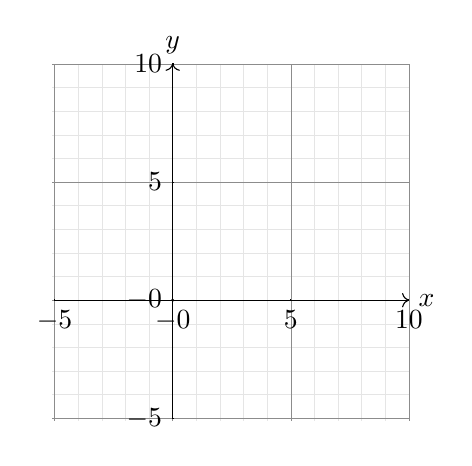
\begin{tikzpicture}[scale=0.3]
    % Draw grid lines
    \draw[step=1cm,gray!20,very thin] (-5.1,-5.1) grid (10,10);
    \draw[step=5cm,gray!90,very thin] (-5.1,-5.1) grid (10,10);
    % Draw x-axis
    \draw[->] (-5,0) -- (10,0) node[right] {$x$};
    % Draw y-axis
    \draw[->] (0,-5) -- (0,10) node[above] {$y$};
    % Draw x-axis labels
    \foreach \x in {-5,-0, 5,10}
        \draw (\x cm,1pt) -- (\x cm,-1pt) node[anchor=north] {$\x$};
    % Draw y-axis labels
    \foreach \y in {-5,-0, 5,10}
        \draw (1pt,\y cm) -- (-1pt,\y cm) node[anchor=east] {$\y$};
    % Draw origin
    \fill (0,0) circle (2pt);
\end{tikzpicture}


\end{minipage}

\part Using your sketch and the domain of the inverse, or otherwise, determine a maximal domain and range of $g$ for which it is bijective.
\fillwithdottedlines{20mm}

\end{parts}


\vfill



\question \textbf{Bonus.} Calculate the inverse of $h: x \mapsto \frac{ax+b}{cx+d}$. What condition is needed on the parameters?



\end{questions}

\begin{tcolorbox}

\textbf{Name of marker:}

\begin{center}
\gradetable[h][questions]
\end{center}

\end{tcolorbox}


\end{document}